\documentclass[a4paper, 10pt, final, garamond]{book}
\usepackage{cours-preambule}

\titleformat{\item}{}{\arabic{item})}{.5em}{}{}
\titleformat{\subitem}{}{\arabic{item}) \alph{subitem} --}{.5em}
{}{}

\makeatletter
\renewcommand{\@chapapp}{Devoir surveill\'e -- num\'ero}
\makeatother

\begin{document}
\setcounter{chapter}{1}

\chapter{Commentaires sur le DS n\degree02}

\section{Commentaires généraux}


% \begin{tcb}[bld,cnt,fontupper=\Large](impo){Points clés}
% 	\begin{itemize}
% 		\item Les interrupteurs, ouverts ou fermés, ne sont PAS des résistances~!
% 		\item Interrupteur fermé (fil) $\Ra i \neq 0, u = 0$~;
% 		\item Interrupteur ouvert $\Ra i=0, u \neq 0$~!
% 		\item Condition initiale $\cancel{\Lra}$ en $t=0$, mais en $t$ initial~!
% 	\end{itemize}
% \end{tcb}

% \begin{center}
% 	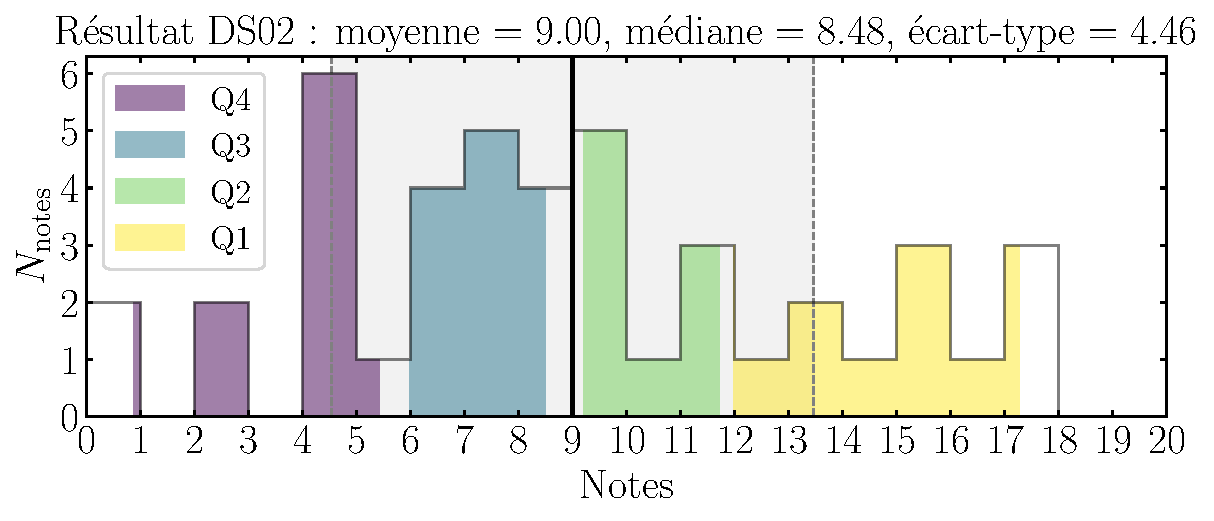
\includegraphics[width=.7\linewidth]{DS02_rslt.pdf}
% \end{center}

\setcounter{section}{0}
\section[24]"E"{Circuit de résistances}

\begin{enumerate}[label=\sqenumi]
	\item[n]{5}% Q1
	\item[n]{4}% Q2
	\item[n]{4}% Q3
	\item[n]{6}% Q4
	\item[n]{5}% Q5
\end{enumerate}

\section[47]"P"{Alimentation d'un train}
\begin{enumerate}[label=\sqenumi]
	\item[n]{3}% Q1
	\item[n]{2}% Q2
	\item[n]{5}% Q3
	\item[n]{4}% Q4
	\item[n]{3}% Q5
	\item[n]{3}% Q6
	\item[n]{2}% Q7
	\item[n]{4}% Q8
	\item[n]{6}% Q9
	\item[n]{7}% Q10
	\item[n]{2}% Q11
	\item[n]{4}% Q12
	\item[n]{2}% Q13
\end{enumerate}

\section[68]"P"{Étude d'une lampe de secours rechargeable}
\begin{enumerate}[label=\sqenumi]
	\item[n]{10}% Q1
	\item[n]{3}% Q2
	\item[n]{4}% Q3
	\item[n]{14}% Q4
	\item[n]{6}% Q5
	\item[n]{8}% Q6
	\item[n]{7}% Q7
	\item[n]{6}% Q8
	\item[n]{7}% Q9
	\item[n]{3}% Q10
\end{enumerate}

\section[71]"P"{Guirlandes électriques}
\begin{enumerate}[label=\sqenumi]
	\item[n]{2}% Q1
	\item[n]{6}% Q2
	\item[n]{5}% Q3
	\item[n]{3}% Q4
	\item[n]{2}% Q5
	\item[n]{3}% Q6
	\item[n]{3}% Q7
	\item[n]{2}% Q8
	\item[n]{3}% Q9
	\item[n]{5}% Q10
	\item[n]{5}% Q11
	\item[n]{8}% Q12
	\item[n]{7}% Q13
	\item[n]{6}% Q14
	\item[n]{2}% Q15
	\item[n]{5}% Q16
	\item[n]{2}% Q17
	\item[n]{2}% Q18
\end{enumerate}

\end{document}
